\documentclass[problem]{mcs}

\begin{pcomments}
  \pcomment{MQ_a_baseball_series}
  \pcomment{from: S09.cp12r}
\end{pcomments}

\pkeywords{
  probability
}

%%%%%%%%%%%%%%%%%%%%%%%%%%%%%%%%%%%%%%%%%%%%%%%%%%%%%%%%%%%%%%%%%%%%%
% Problem starts here
%%%%%%%%%%%%%%%%%%%%%%%%%%%%%%%%%%%%%%%%%%%%%%%%%%%%%%%%%%%%%%%%%%%%%

% F09, S09

\begin{problem}
{\bf [A Baseball Series]} \\
The New York Yankees and the Boston Red Sox are playing a
two-out-of-three series.  (In other words, they play until one team
has won two games.  Then that team is declared the overall winner and
the series ends.)  Assume that the Red Sox win each game with
probability $2/3$, regardless of the outcomes of previous games.

Answer the questions below using the four step method.  You can use
the same tree diagram for all three problems.

\bparts

\ppart What is the probability that only 2 games are played? 

\begin{center}
\exambox{0.7in}{0.4in}{0.2in}
\end{center}
\begin{solution}
This means that either the Yankees win both games, which occurs with probability 
$(1/3)^2$ or the Red Sox win both games, which occurs with probability $(2/3)^2$.

Summing these yields $(1/3)^2+(2/3)^2 = 5/9$

\end{solution}
\ppart What is the probability that the winner of the series loses the
first game?

\begin{center}
\exambox{0.7in}{0.4in}{0.2in}
\end{center}
\begin{solution}
We use the four step method with the graph below.
\end{solution}

\ppart What is the probability that the Red Sox loses the
series?

\begin{center}
\exambox{0.7in}{0.4in}{0.2in}
\end{center}

\eparts

\begin{solution}
A tree diagram is worked out below.
%
\begin{center}
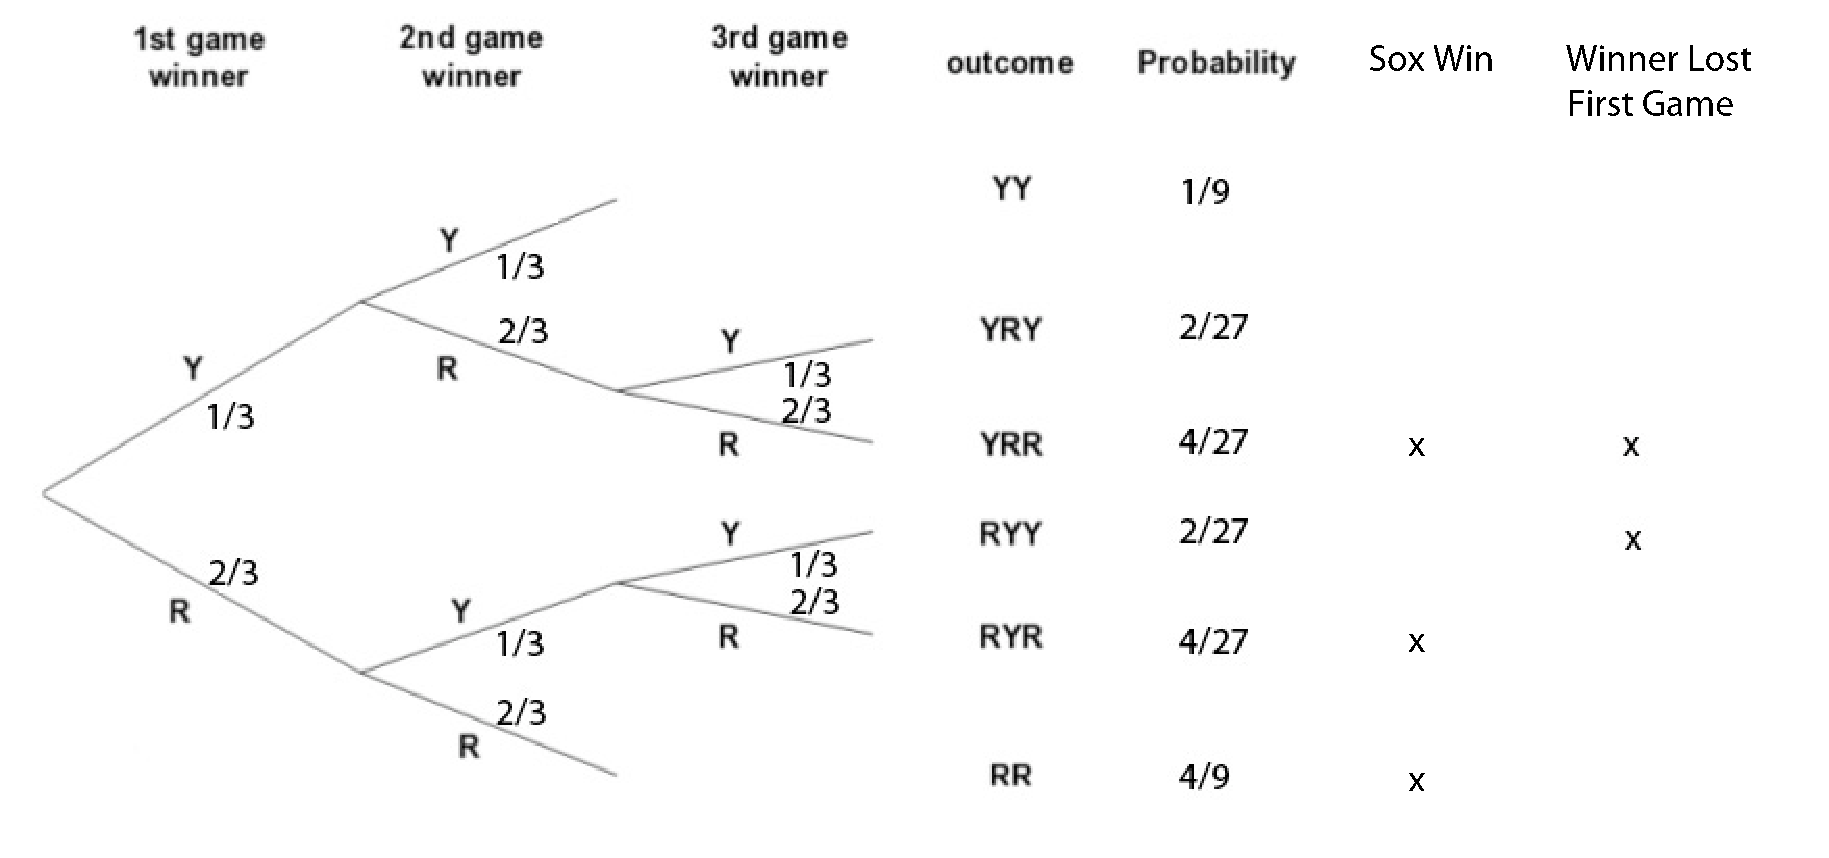
\includegraphics[width=6.25in]{figures/series3.pdf}
\end{center}
%
From the tree diagram, we get:
%
\begin{align*}
\pr{\text{Winner Lost First Game}}
    & = \frac{4}{27} + \frac{2}{27}}
      = \frac{6}{27} \\
\pr{\text{Sox Lost}}
    & = \frac{3}{27} + \frac{2}{27} + \frac{2}{27}}
      = \frac{7}{27} \\

\end{align*}

\end{solution}

\end{problem}

%%%%%%%%%%%%%%%%%%%%%%%%%%%%%%%%%%%%%%%%%%%%%%%%%%%%%%%%%%%%%%%%%%%%%
% Problem ends here
%%%%%%%%%%%%%%%%%%%%%%%%%%%%%%%%%%%%%%%%%%%%%%%%%%%%%%%%%%%%%%%%%%%%%

\endinput